\documentclass[a4paper,10pt]{jsarticle}

% レイアウト
\setlength{\textwidth}{\fullwidth}
\setlength{\textheight}{39\baselineskip}
\addtolength{\textheight}{\topskip}
\setlength{\voffset}{-0.5in}
\setlength{\headsep}{0.3in}
\pagestyle{myheadings}

% パッケージ
\usepackage[dvipdfmx]{graphicx}
\usepackage{amsmath,amssymb,epsfig}
\usepackage{bm}
\usepackage{ascmac}
\usepackage{pifont}
\usepackage{multirow}
\usepackage{enumerate}
\usepackage{cases}
\usepackage{type1cm}
\usepackage{cancel}
\usepackage{url}
\usepackage{listings,jlisting}
% 大きな中括弧
\usepackage{cases}

% 定義
\DeclareMathOperator*{\argmin}{arg\,min}
\DeclareMathOperator*{\argmax}{arg\,max}
\def\vec#1{\mbox{\boldmath$#1$}}
\def\R{{\Bbb R}}

% カウンタの設定
\setcounter{section}{0}
\setcounter{subsection}{0}
\setcounter{subsubsection}{0}
\setcounter{equation}{0}

% キャプションの図をFigに変更
\renewcommand{\figurename}{Fig.}
\renewcommand{\tablename}{Tab.}

% 式番号を式(章番号.番号)に
\makeatletter
\renewcommand{\theequation}{\arabic{section}.\arabic{equation}}
\@addtoreset{equation}{section}
\makeatother

% 表紙
\title{知能システム学特論レポート}
\author{
(DL2班)Caffe on Ubuntu\\
}
\date{2015年\ 7月\ 2日}

% ドキュメントの開始
\begin{document}
\maketitle
\section{報告者}
\begin{list}{}{}
 \item 15344203\hspace{0.5cm} 有田 裕太
 \item 15344206\hspace{0.5cm} 緒形 裕太
 \item 15344209\hspace{0.5cm} 株丹 亮
 \item 12104125\hspace{0.5cm} 宮本 和
\end{list}

\section{進行状況}

\begin{itemize}
\item 理論研究
\item 中間層の出力
\end{itemize}

\section{理論研究}
\subsection{畳込みニューラルネットワーク}
畳込みニューラルネットワークは主に画像認識に応用される順伝播型ニューラルネットワークである.
順伝播型ネットワークは隣接層間のユニットの全てが結合されているのに対し,畳込みニューラルネットワークでは特定のユニットのみが結合を持つ特別な構造を持つ.
そして,畳込みとプーリングという画像処理の基本的な演算を行う.
これは生物の脳の視覚野に関する神経科学の知見をヒントにしている.
神経細胞はその受容野に刺激が入った場合にのみ反応し,受容野の外側にいくら刺激を与えても,細胞を発火しないという特徴を持つ.

\begin{figure}[htbp]
 \begin{minipage}{0.5\hsize}
  \begin{center}
   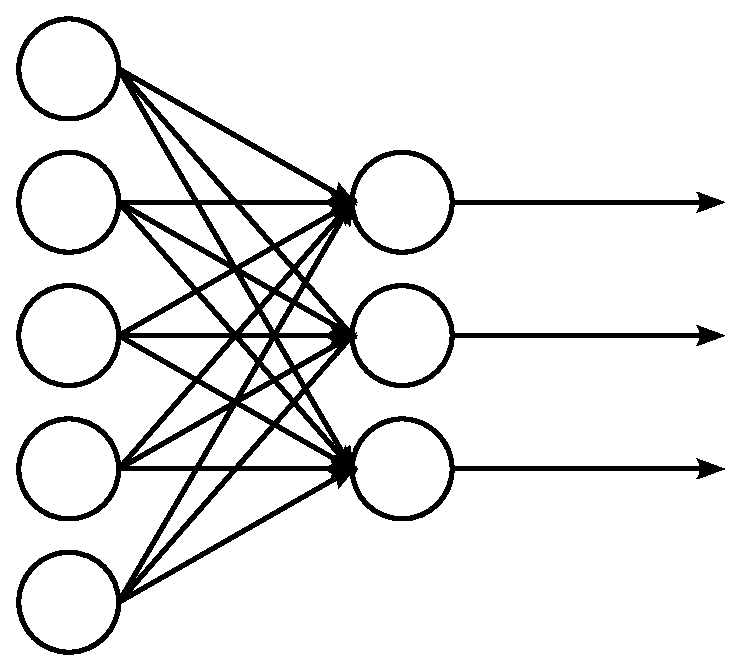
\includegraphics[width=40mm]{fig/eps/FNN.eps}
  \end{center}
  \caption{順伝播型ニューラルネットワーク}
  \label{fig:FNN}
 \end{minipage}
 \begin{minipage}{0.5\hsize}
  \begin{center}
   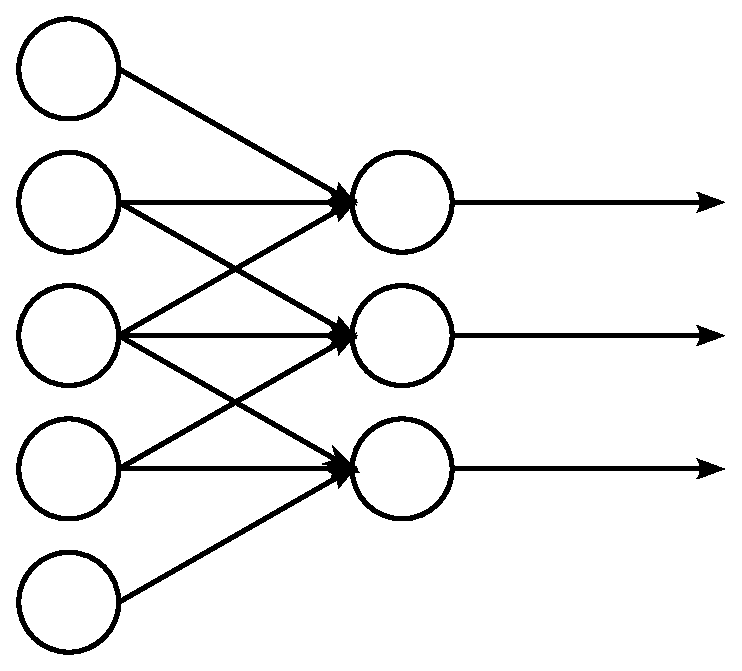
\includegraphics[width=40mm]{fig/eps/CNN.eps}
  \end{center}
  \caption{畳込みニューラルネットワーク}
  \label{fig:CNN}
 \end{minipage}
\end{figure}

\subsection{単純型細胞と複雑型細胞}
単純型細胞と複雑型細胞のモデルをFig.~\ref{fig:単純型細胞と複雑型細胞のモデル}に示す.(a),(b)は$4\times4$の入力層が中間層のそれぞれと結合していることを示しており,
(c),(d)は入力パターンの位置変化に伴う中間層および出力層の状態の変化を示している.

中間層は単純型細胞,出力層は複雑型細胞のモデルとなっており,中間層は位置選択性が厳密であるが,出力層は入力パターンが少しずれても活性化する.
全体への入力が(c)から(d)のように変化すると,中間層でも図のように活性化するユニットが変化するが,出力層のユニットは活性化したままである.
これは出力層は中間層のユニットが一つでも活性化されていれば活性化するためである.

この2つの細胞をモデル化した二層構造のペアを繰り返す構造が畳み込みニューラルネットに用いられている.
物体カテゴリ認識は長年コンピュータには難しいとされてきたが,近年畳み込みニューラルネットによってそれも解決されつつある.
神経科学の分野では,多層の畳み込みニューラルネットが霊長類の脳の高次視覚野と似た振る舞いを示すことが示されている.

\begin{figure}[t]
 \centering
 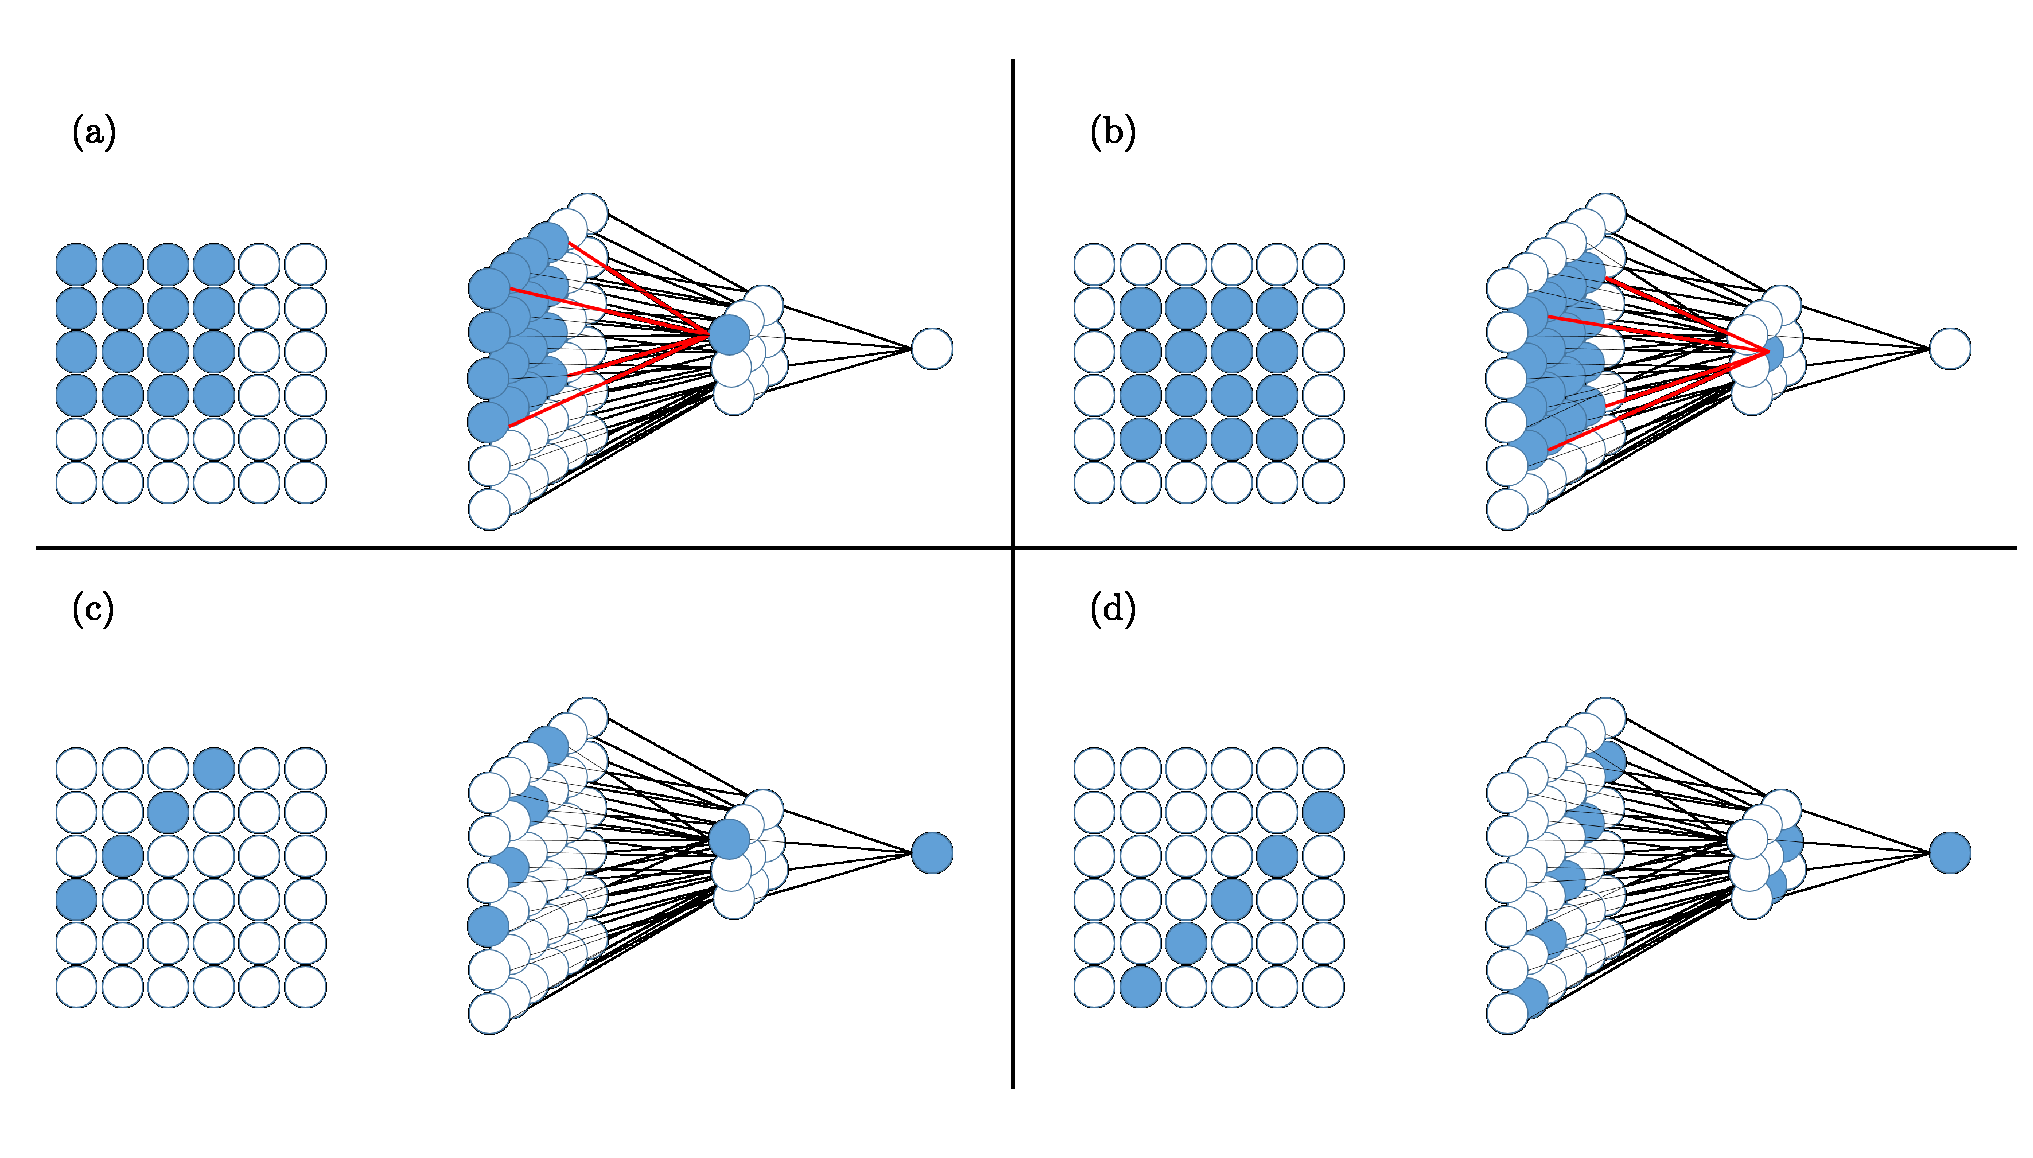
\includegraphics[scale=0.4]{fig/eps/cnn62.eps}
  \caption{単純型細胞と複雑型細胞のモデル}
  \label{fig:単純型細胞と複雑型細胞のモデル}
\end{figure}

\subsection{全体の構造}
物体の認識などの画像認識でよく用いられる畳込みネットの典型的な構造をFig.~\ref{fig:畳込みネットの構造}に示す.
入力側から出力側に向けて,畳込み層(convolution layer)とプーリング層(pooling layer)がペアでこの順に並び,このペアが複数回繰り返される.
特に畳込み層とプーリング層のペアの一回操作で行われる手順の一例をFig.~\ref{fig:畳込み層とプーリング層の操作}に示す.
\begin{figure}[t]
 \centering
 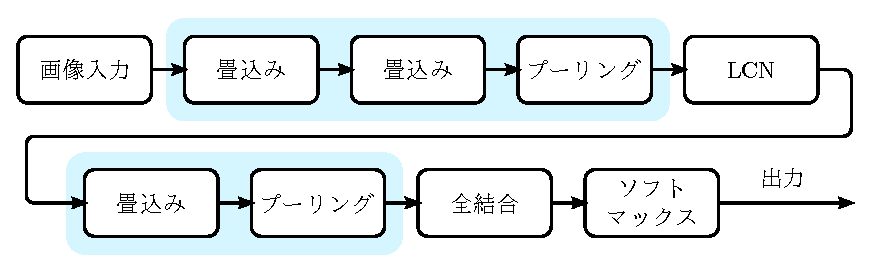
\includegraphics[scale=0.65]{fig/eps/structure.eps}
  \caption{畳込みネットの構造}
  \label{fig:畳込みネットの構造}
\end{figure}
\begin{figure}[t]
 \centering
 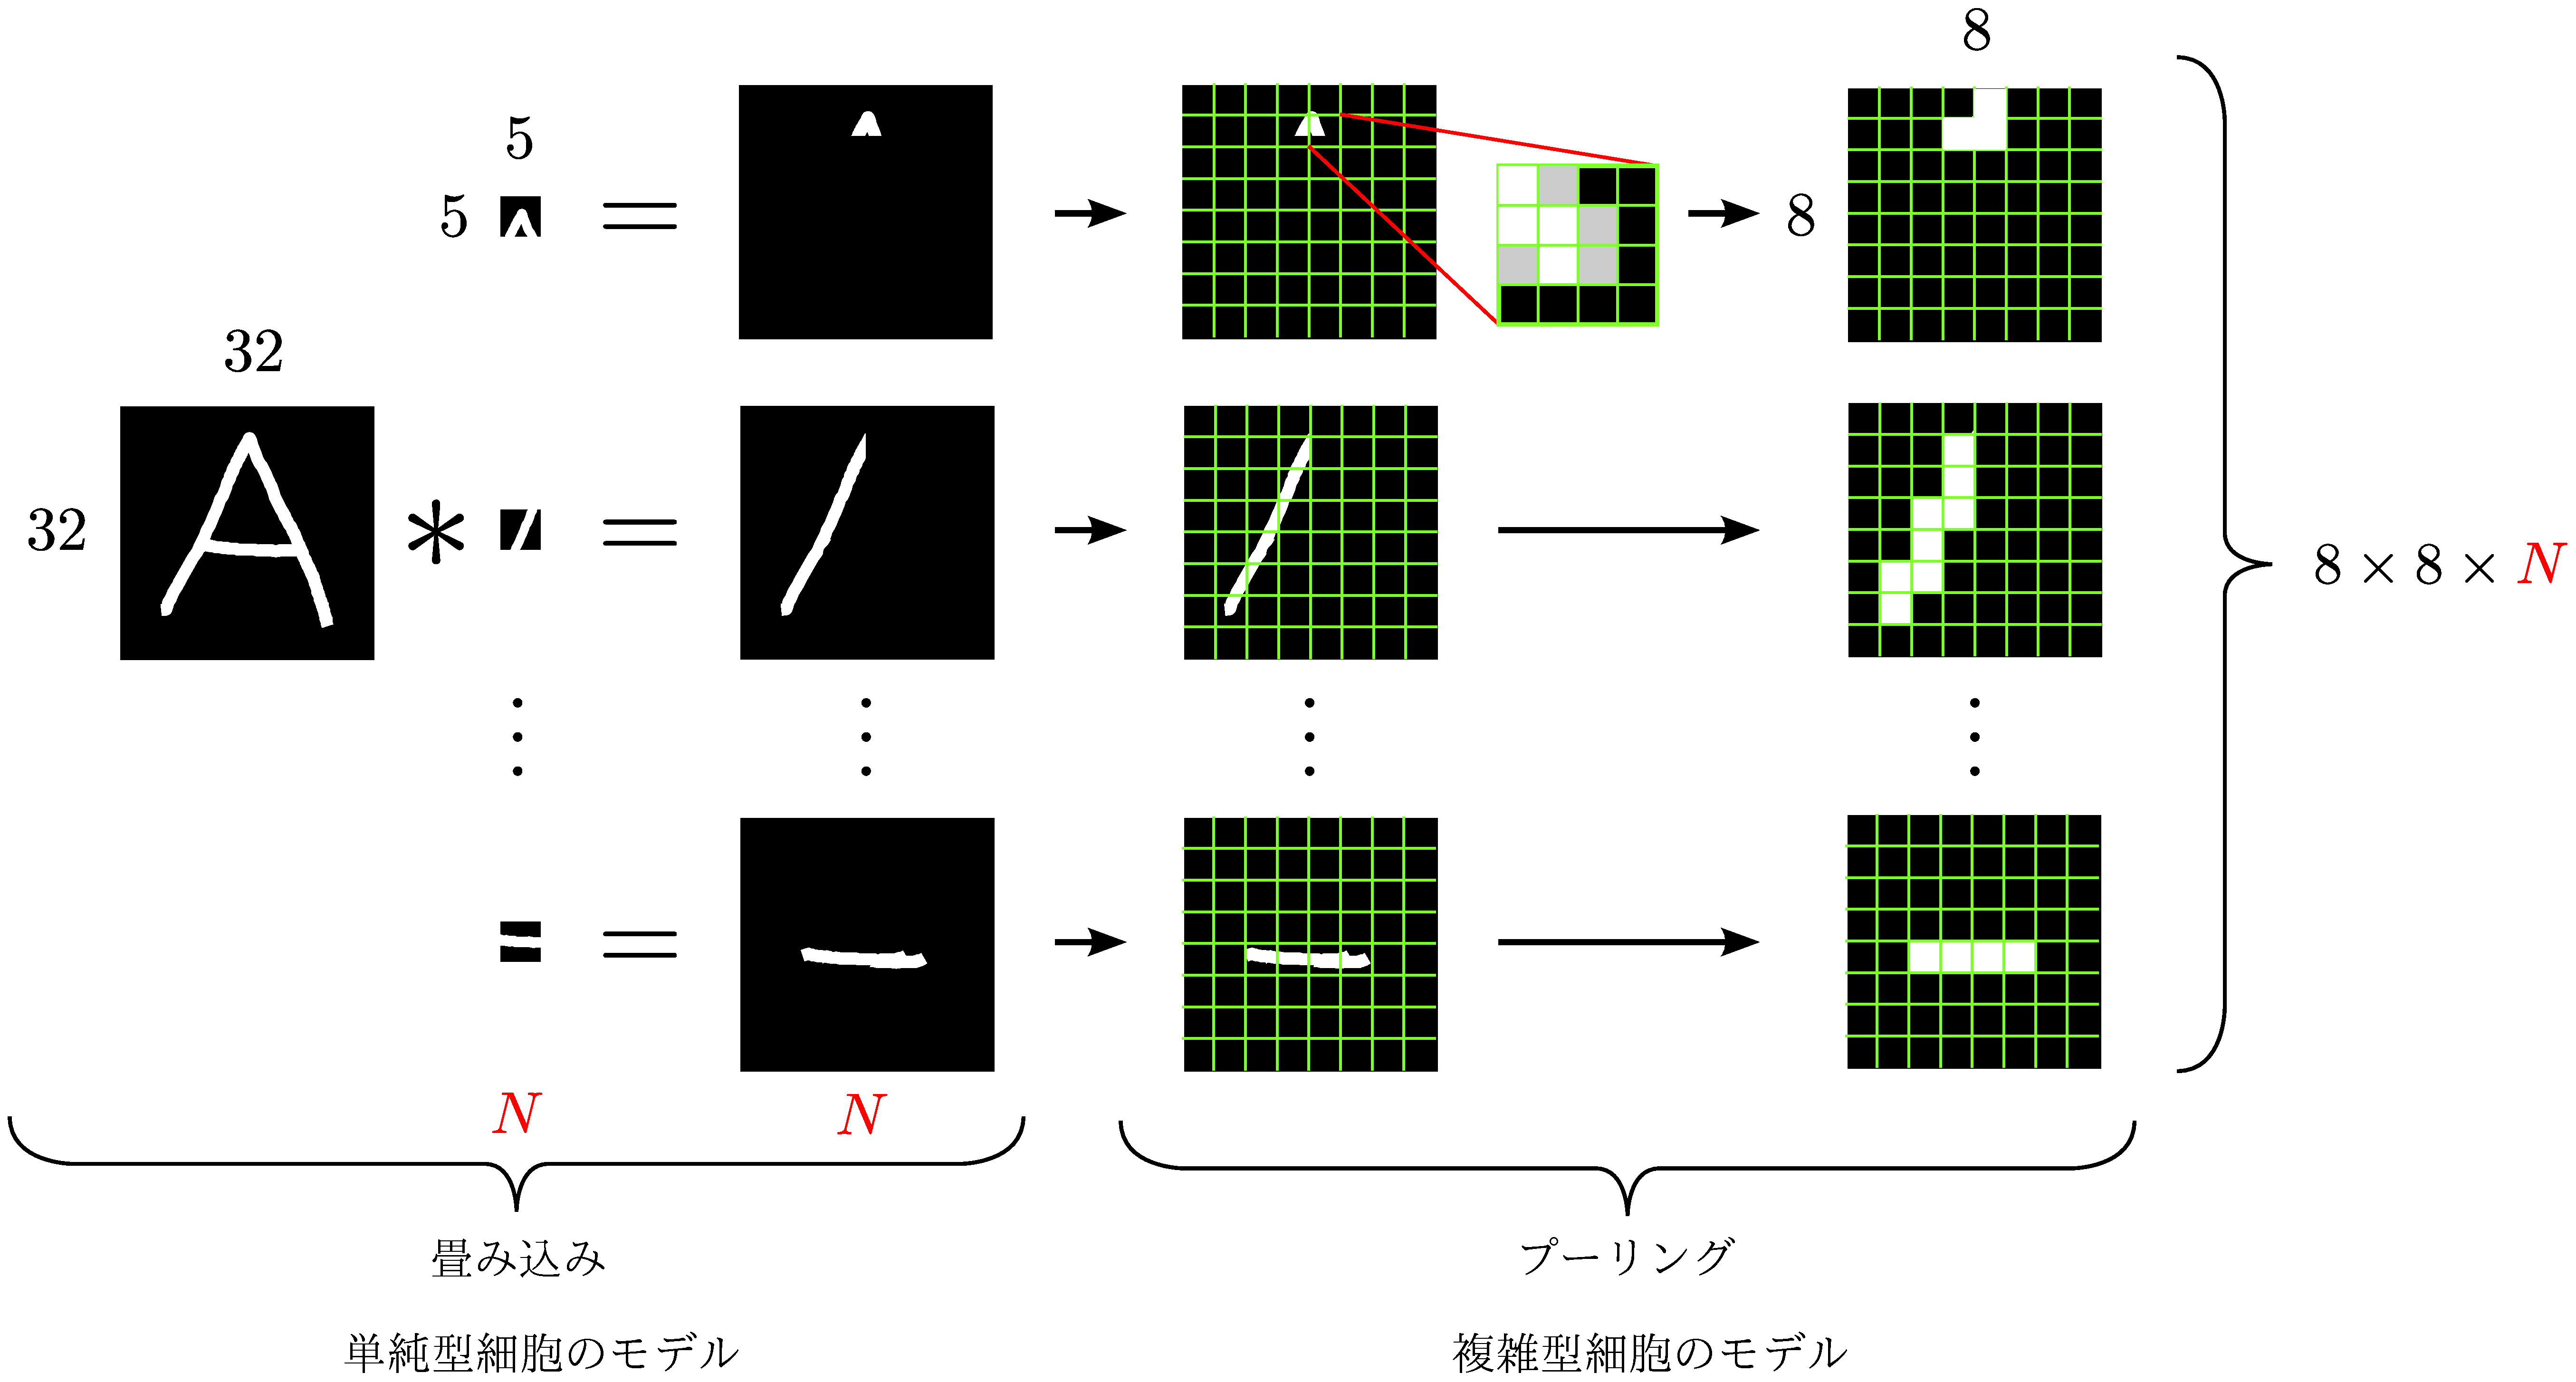
\includegraphics[width=140mm]{fig/eps/conv_pool.eps}
  \caption{畳込み層とプーリング層の操作}
  \label{fig:畳込み層とプーリング層の操作}
\end{figure}
また畳込み層とプーリング層の後に,局所コントラスト正規化(local contrast normalization, LCN)層を挿入する場合がある.

そして畳込み層とプーリング層の繰り返しの後には,隣接層間ユニットが全結合した層が配置される.
これを全結合層(fully-connected layer)と呼ぶ.
全結合層は順伝播型ネットワークの各層と同じで,目的がクラス分類であれば最終的な出力はソフトマックスを適用する.


\section{プログラム}
\subsection{caffeNetの構造}
caffeでは訓練済みのニューラルネットワークをダウンロードし,使用することができる.先日,示したサンプルの画像認識に用いたCNNの構造をFig.\ref{204941_1Jul15}に示す.
赤色は畳込み層,オレンジ色はプーリング層,青色は正規化層,紫色は全結合層を表している.また,活性化関数にはソフトマックス関数を用いている.すなわち,このCNNは5つの畳込み層,3つのプーリング層,2つの正規化層,そして3つの全結合層からできている.

Fig.\ref{204941_1Jul15}を出力するには,caffeのディレクトリ直下で,次のコマンドを実行する.
\begin{lstlisting}[basicstyle=\ttfamily\footnotesize, frame=single,breaklines = true]
python/draw_net.py models/bvlc_reference_caffenet/train_val.prototxt caffeNet.png --rankdir BT
\end{lstlisting}

\begin{figure}[p]
 \centering
 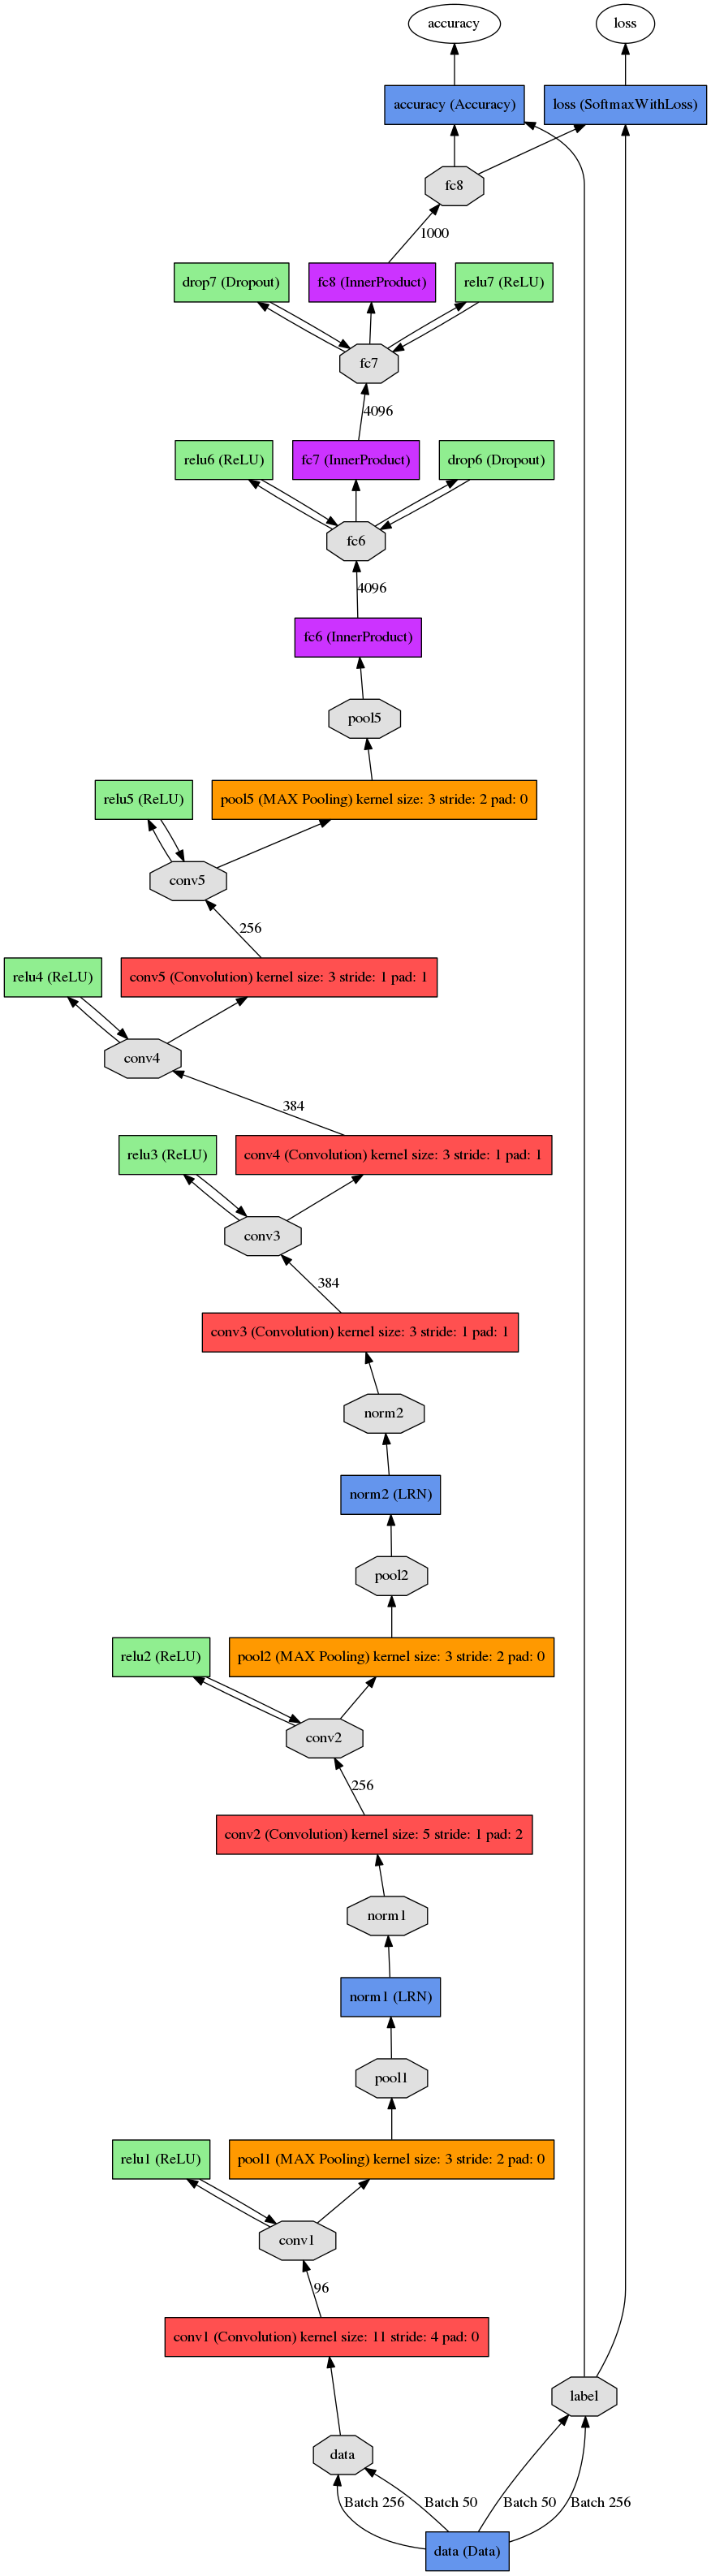
\includegraphics[scale=0.2]{fig/png/caffeNet.png}
  \caption{caffeNet}
  \label{204941_1Jul15}
\end{figure}

\subsection{中間層の出力}
畳込み1層目のフィルタとFig.に示す入力画像を入力したときの出力を得ることができた.1層目のフィルタをFig.\ref{220453_1Jul15},その出力をFig.\ref{220458_1Jul15}に示す.
畳込み1層目は全部で96個の$11\times11$のフィルタから構成されており,ストライドが4である.従って,出力される画像のサイズは$55\times55$であり,96個の画像が出力される.
\begin{figure}[b]
 \centering
 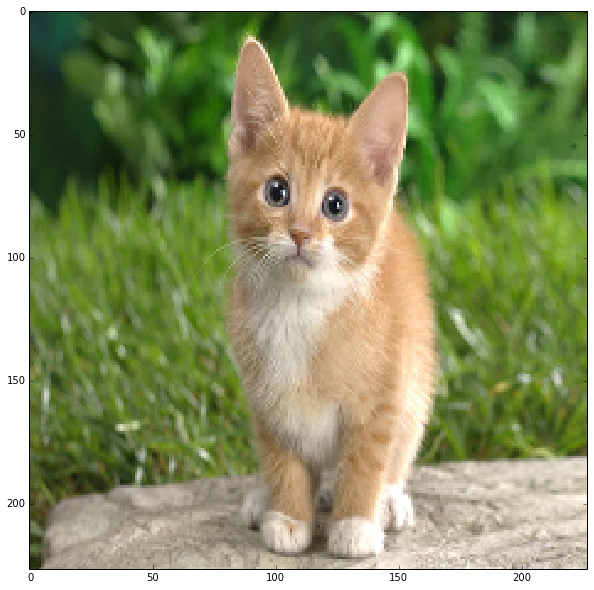
\includegraphics[scale=0.5]{fig/png/input.png}
  \caption{入力画像}
\end{figure}
\begin{figure}[t]
 \centering
 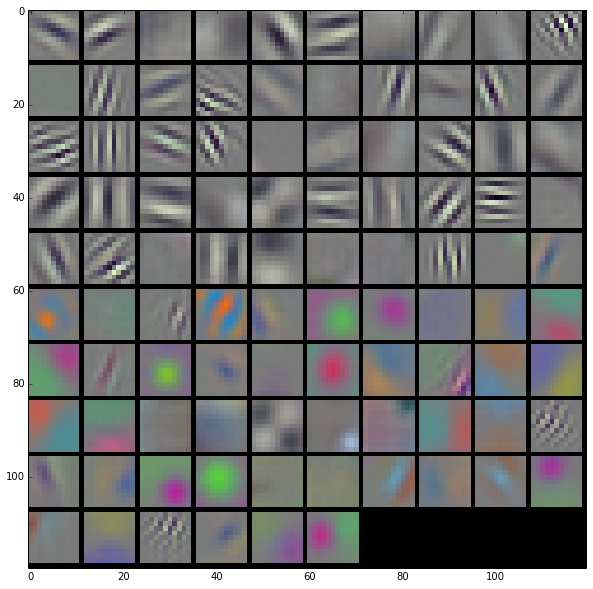
\includegraphics[scale=0.4]{fig/png/conv1_params.png}
  \caption{畳込み層1層目のフィルタ}
  \label{220453_1Jul15}
\end{figure}
\begin{figure}[t]
 \centering
 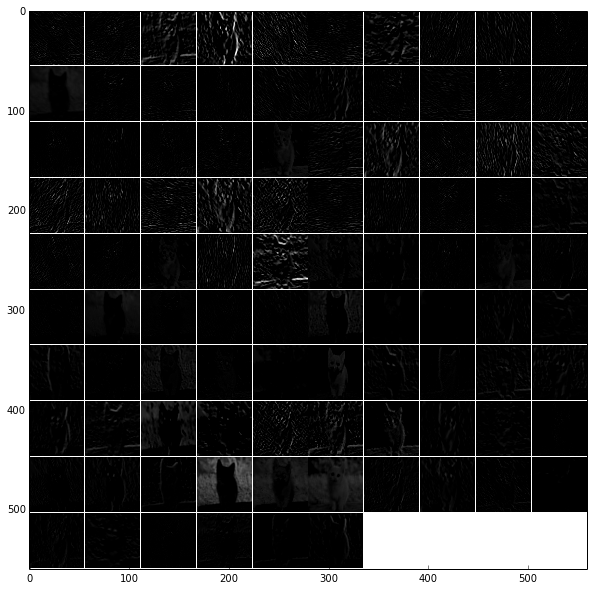
\includegraphics[scale=0.4]{fig/png/conv1_blobs.png}
  \caption{畳込み層1層目のフィルタ出力}
  \label{220458_1Jul15}
\end{figure}
中間層を表示するにあたりipython notebookを用いた.
\section{今後の課題}
\begin{itemize}
 \item CNNの詳細な調査
 \item 畳み込み,プーリングの理論
 \item データセットの作成
\end{itemize}


\begin{thebibliography}{99}
  \addcontentsline{toc}{section}{参考文献}
 \bibitem{okatani} 岡谷貴之,``機械学習プロフェッショナルシリーズ 深層学習'',講談社,2015.
 \end{thebibliography}

\end{document}